\input{mmd-beamer-header-11pt}
\def\mytitle{Part 3: An introduction to Bayesian inference}
\def\mydate{25 March 2015}
\def\myauthor{Matthew Pitkin}
\def\affiliation{University of Glasgow}
\def\latexxslt{beamer}
\def\latexmode{beamer}
\def\event{GraWIToN School}
\def\theme{m}
\input{mmd-beamer-begin-doc}


% Part 3 of my lecture course on statistics for the GraWIToN school
%
% Introduction to Bayesian inference


\begin{frame}

\frametitle{Overview}
\label{overview}

In this part of the course we will discuss

\begin{itemize}
\item parameter estimation

\item hypothesis testing

\end{itemize}

from a Bayesian perspective.

\end{frame}

\begin{frame}

\frametitle{Frequentist vs. Bayesian approach}
\label{frequentistvs.bayesianapproach}

Recall that:

\begin{itemize}
\item Frequentist

\begin{itemize}
\item data are a \textbf{repeatable} random sample

\item parameters \textbf{remain fixed} during this repeatable process

\end{itemize}

\item Bayesian

\begin{itemize}
\item data are an \textbf{observation from the realised sample}

\item parameters are unknown and described \textbf{probabilistically}

\end{itemize}

\end{itemize}

\end{frame}

\begin{frame}

\frametitle{The Bayesian approach}
\label{thebayesianapproach}

In the Bayesian approach, we can test our model given our data (e.g. rolls of a die) and see how
our knowledge of its parameters evolve, for any sample size, considering only the data that we \emph{did}
actually observe.

All we need is Bayes theorem:
\[
\redob{p(\text{model}|\text{data},I)}^{\mathclap{\text{Posterior}}} \propto
\redob{p(\text{data}|\text{model},I)}^{\mathclap{\text{Likelihood}}} \times 
\redob{p(\text{model}|I)}^{\mathclap{\text{Prior}}}
\]

\begin{itemize}
\item \textbf{prior}: \emph{what we knew before}

\item \textbf{likelihood}: \emph{the influence of our observations}

\item \textbf{posterior}: \emph{what we know now}

\end{itemize}

\end{frame}

\begin{frame}

\frametitle{A Bayesian example: is a coin fair?}
\label{abayesianexample:isacoinfair}

How can we determine if a coin is fair\footnote{See e.g. Chap. 2 of Sivia~\citep{Sivia}.}? We can consider a large number of contiguous propositions over
the range in which the bias weighting $H$ of the coin might lie:

\begin{itemize}
\item $H = 0$ coin produces a tail every time

\item $H = 1$ coin produces a head every time

\item $H = 0.5$ is a `fair' coin with 50:50 chance of head or tail

\item continuum of probabilities $0 \le H \le 1$

\end{itemize}

Given some data (an observed number of coin tosses) we can assess how much we believe each of
these propositions (e.g. $0 \le H < 0.01$, $0.01 \le H < 0.02$, and so on) to be true, e.g.
\[
\text{Prob}(0 \le H < 0.01|d)
\]

\end{frame}

\begin{frame}

\frametitle{A Bayesian example: is a coin fair?}
\label{abayesianexample:isacoinfair}

In the limiting case where our propositions each lie in the infinitesimal range ${\rm d}H$
our inference about the bias weighting is summarised by the pdf for the conditional probability
$p(H|d,I)$, i.e. the \emph{posterior}. We can use Bayes' theorem to calculate it.

For coin flips, assuming that they are independent events, the probability of obtaining `$r$ heads in
$n$ tosses' is given by the binomial distribution, so our \emph{likelihood} is:
\[
p(d|H,I) \propto H^r(1-H)^{n-r}
\]
But, what should we use as our \emph{prior}?

\end{frame}

\begin{frame}

\frametitle{A Bayesian example: is a coin fair?}
\label{abayesianexample:isacoinfair}

But, what should we use as our \emph{prior}?

Assuming we have no knowledge about the provenance of the coin, or the person tossing it, and want to
reflect total ignorance of the possible bias, then a simple probability reflecting this is a \textbf{uniform},
or \textbf{flat}, pdf:
\[
p(H|I) =
\begin{cases}
1, \text{if } 0 \le H \le 1, \\
0, \text{otherwise}.
\end{cases}
\]
Using these we can calculate our posterior, $p(H|d,I)$, as we obtain more data (counting $r$ as the
number of coin tosses, $n$, increases).

\end{frame}

\begin{frame}

\frametitle{A Bayesian example: is a coin fair?}
\label{abayesianexample:isacoinfair}

\begin{figure}[htbp]
\centering
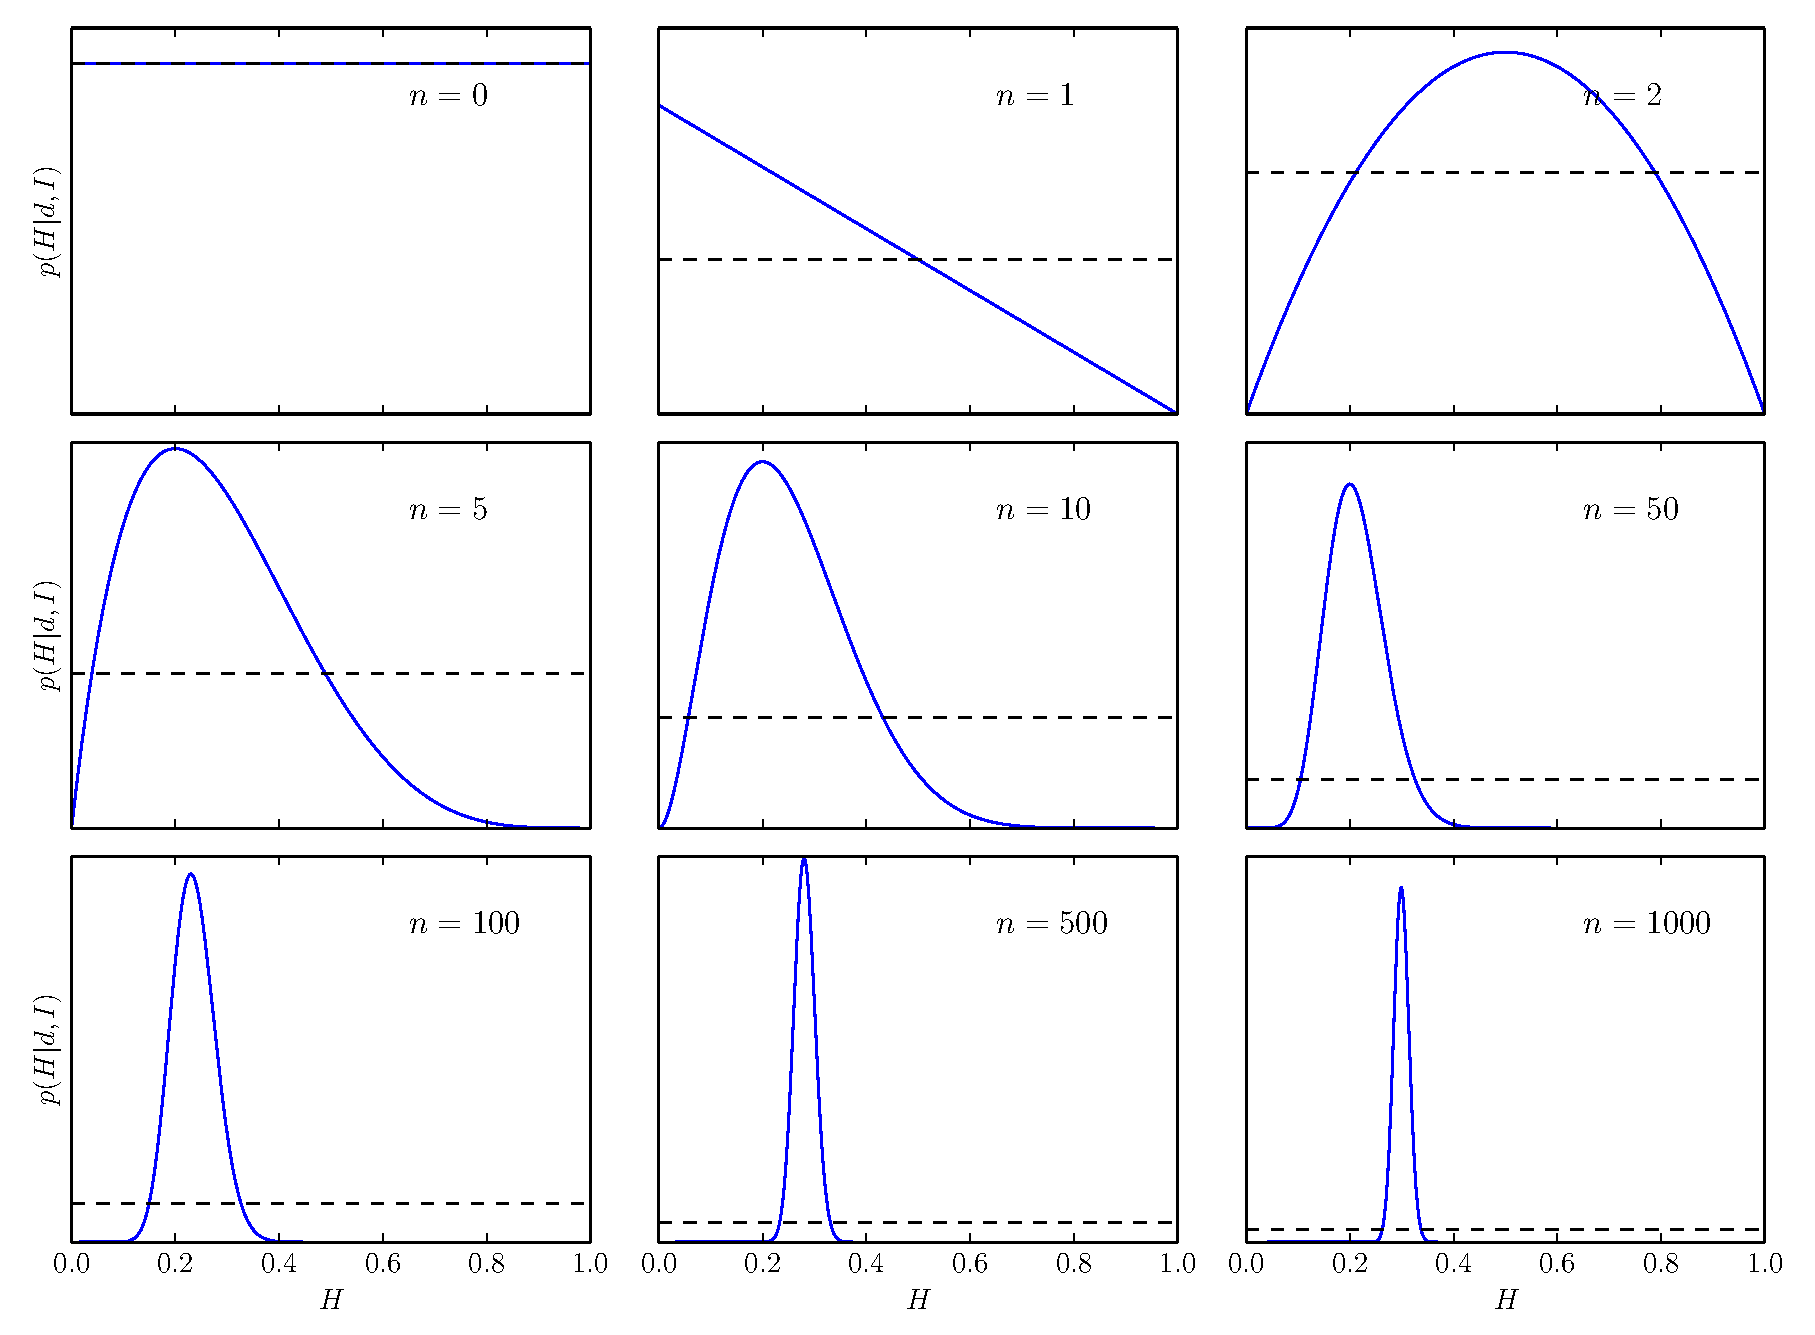
\includegraphics[keepaspectratio,width=\textwidth,height=220pt]{figures/coin_toss.pdf}
\label{coin_toss}
\end{figure}

\end{frame}

\begin{frame}

\frametitle{A Bayesian example: is a coin fair?}
\label{abayesianexample:isacoinfair}

\begin{columns}
    \begin{column}{0.35\textwidth}

As the number of coin tosses increases the posterior evolves from the uniform prior to a tight range in $H$
with the most probable value being $H=0.3$.
\end{column}
\begin{column}{0.65\textwidth}
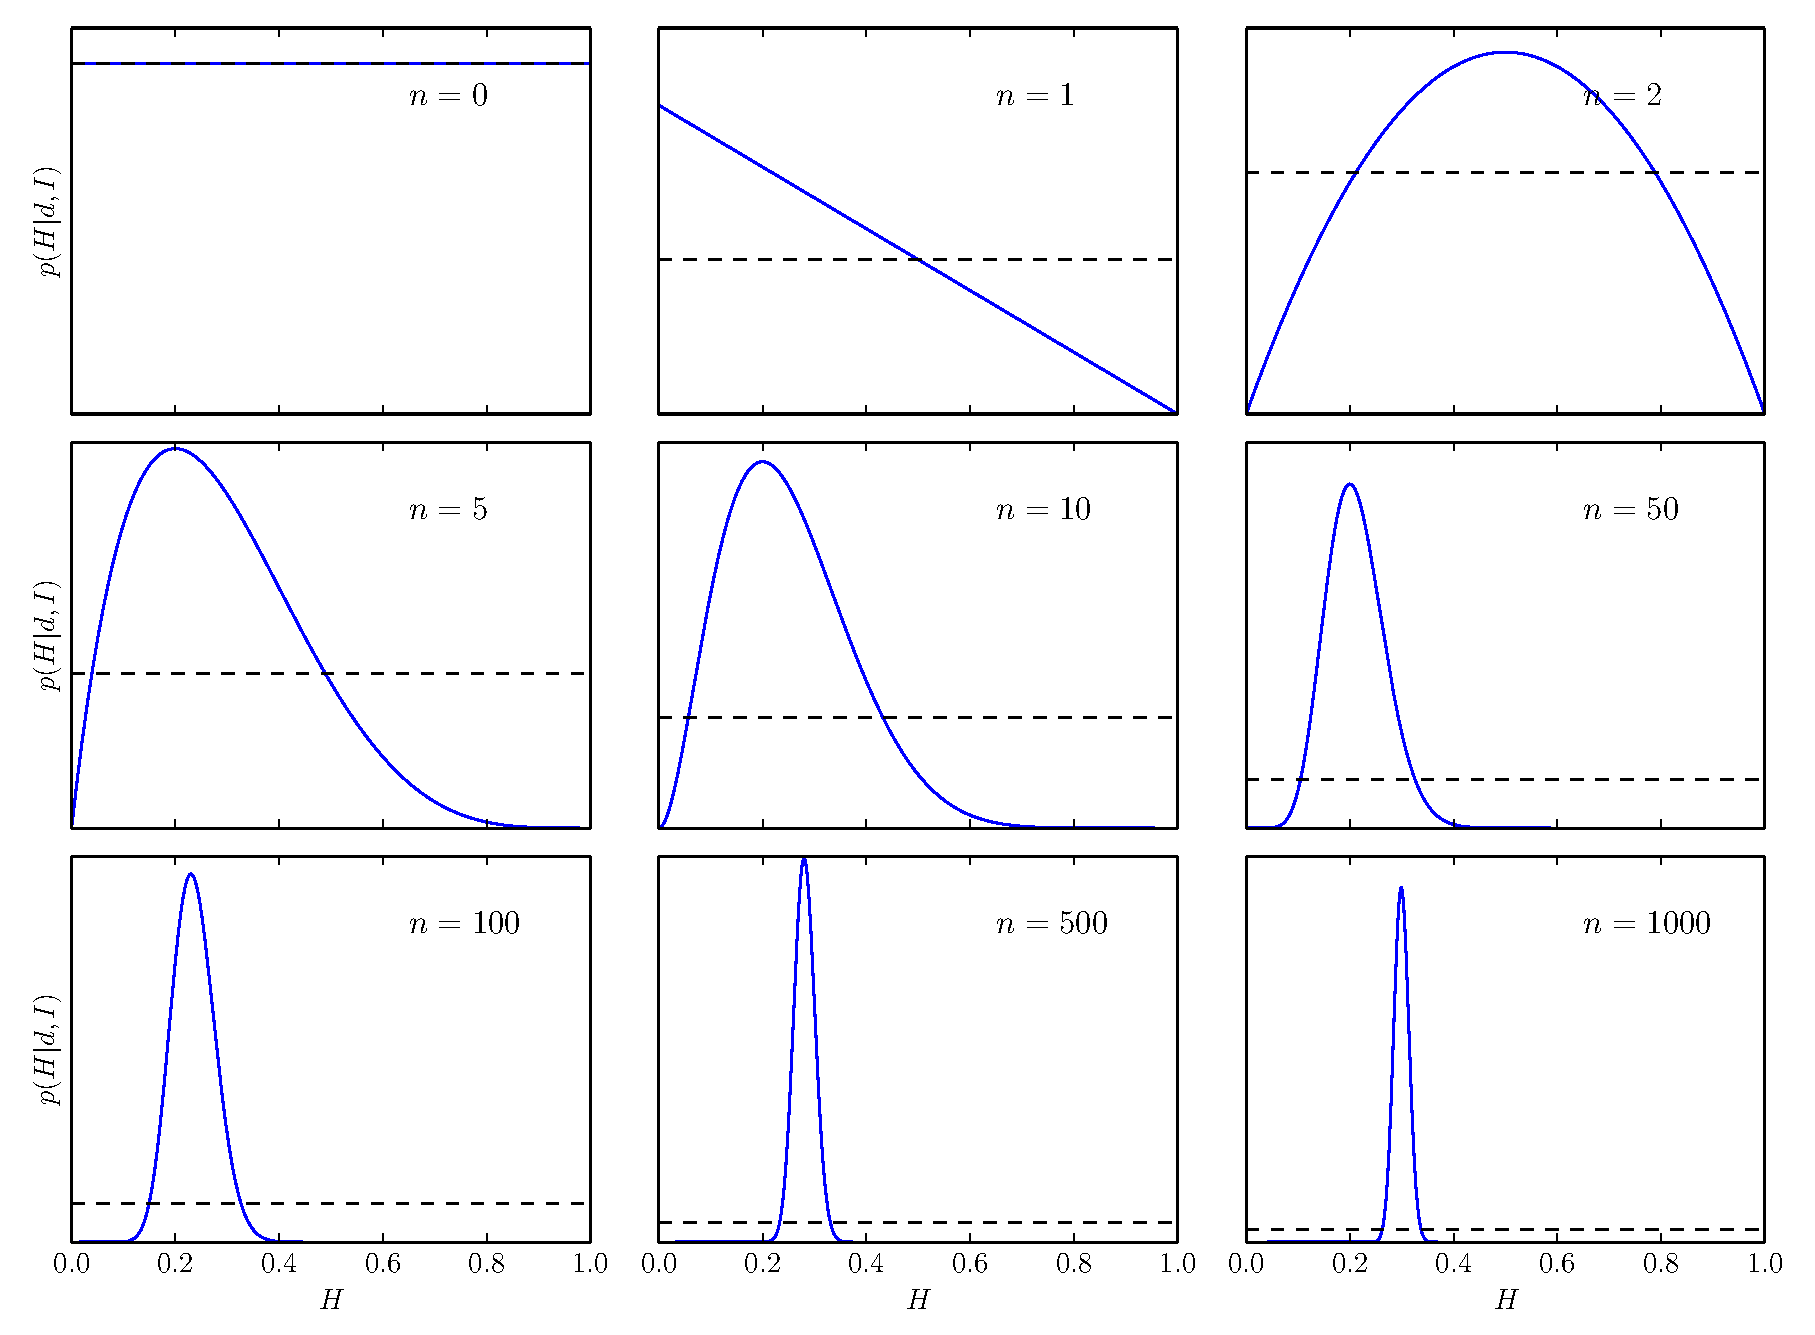
\includegraphics[keepaspectratio,width=\textwidth,height=220pt]{figures/coin_toss.pdf}
\end{column}
\end{columns}

\end{frame}

\begin{frame}

\frametitle{A Bayesian example: is a coin fair?}
\label{abayesianexample:isacoinfair}

What about a \emph{different} prior?

We know that coins are generally fair, so what if we assume this one is too? 

We can assign a Gaussian prior distribution that focusses the probability around the
expected `fair coin' value
\[
p(H|I) \propto \exp{\left(-\frac{1}{2}\frac{(H-\mu_H)^2}{\sigma_H^2}\right)},
\]
with $\sigma_H = 0.05$ and $\mu_H = 0.5$.

\end{frame}

\begin{frame}

\frametitle{A Bayesian example: is a coin fair?}
\label{abayesianexample:isacoinfair}

\begin{figure}[htbp]
\centering
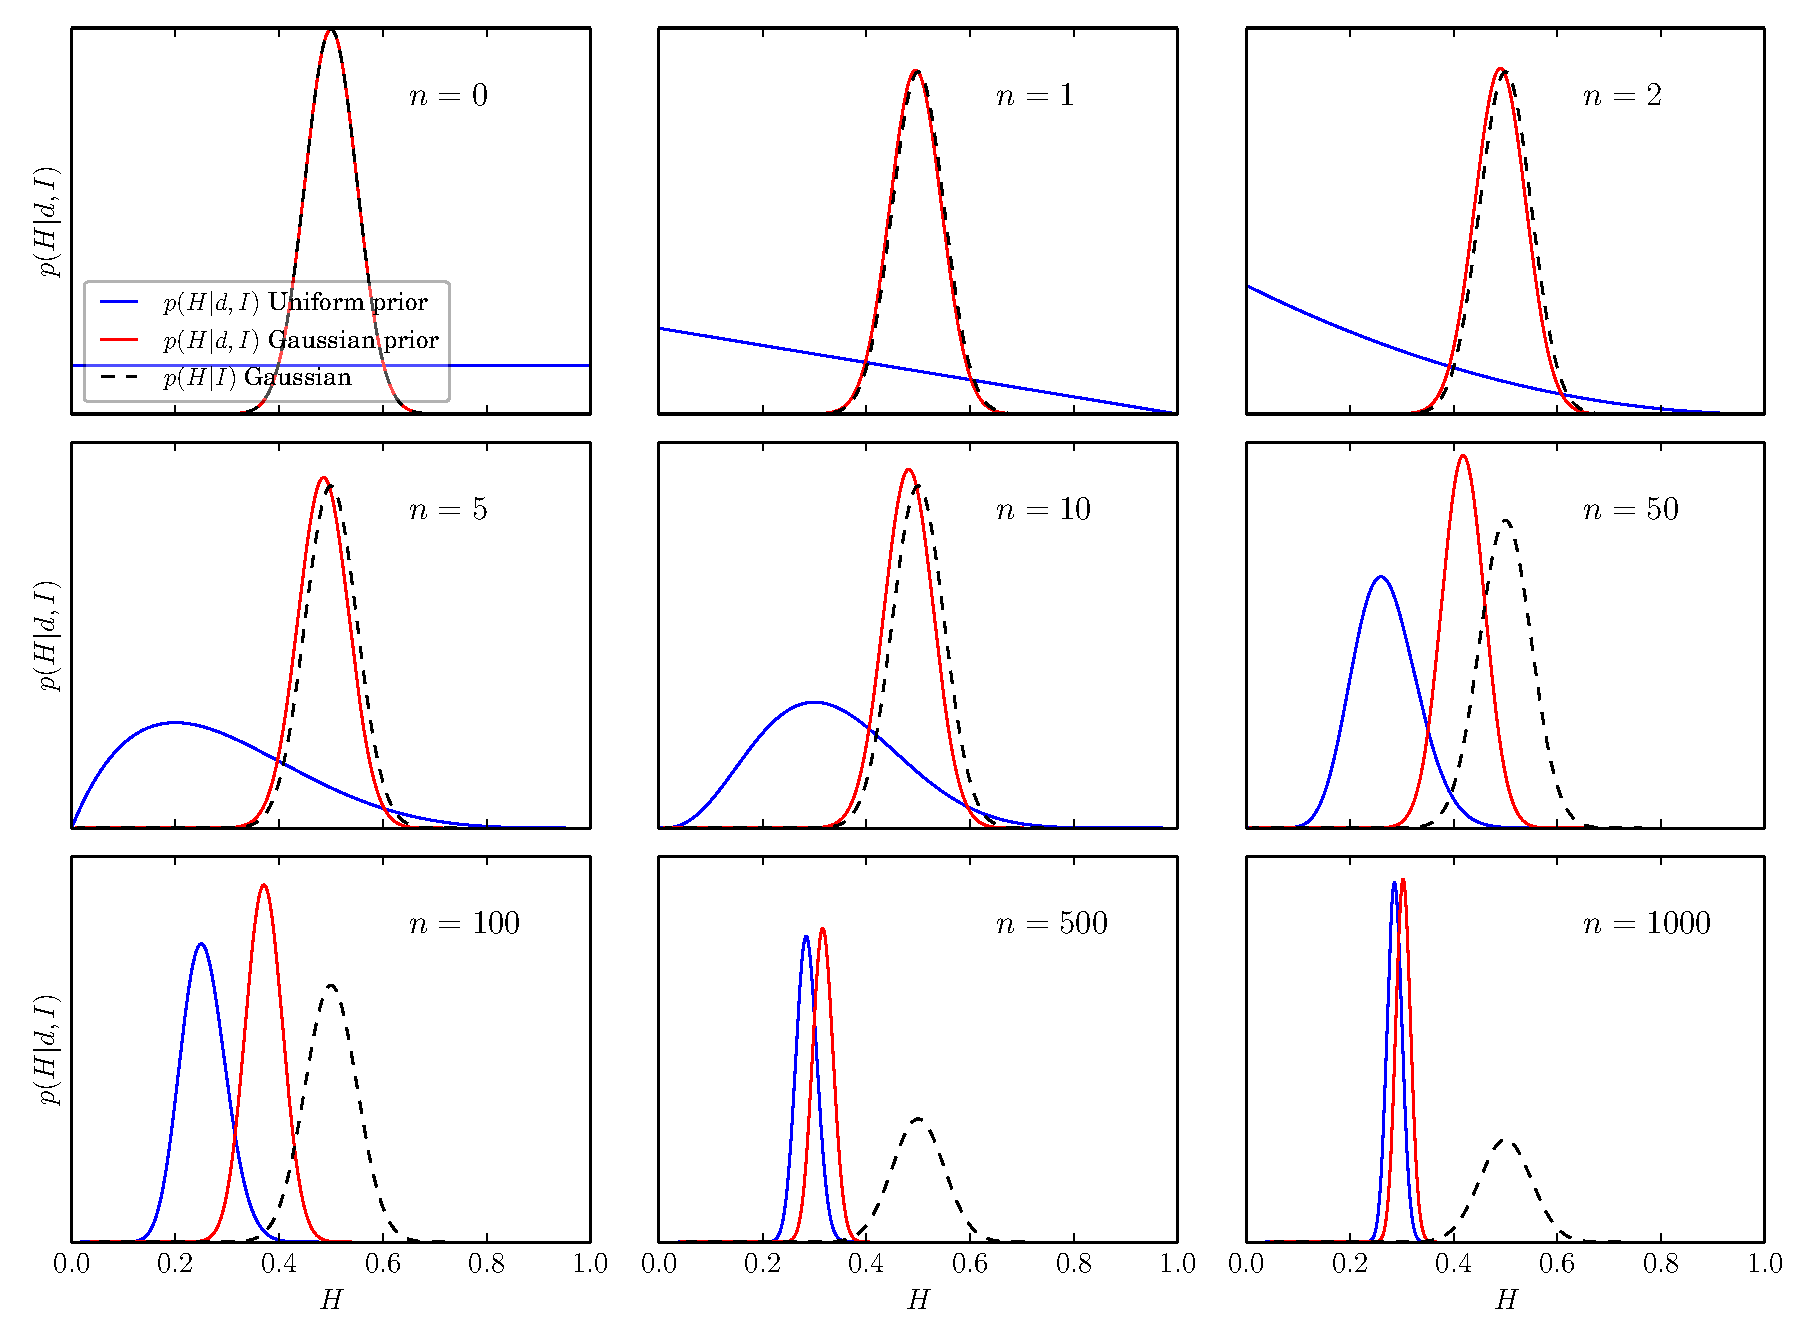
\includegraphics[keepaspectratio,width=\textwidth,height=220pt]{figures/coin_toss_2.pdf}
\label{coin_toss_2}
\end{figure}

\end{frame}

\begin{frame}

\frametitle{A Bayesian example}
\label{abayesianexample}

% New slide 

What do we learn from this?

\begin{itemize}
\item As our data improve (i.e. we gather more samples), the posterior pdf narrows and becomes
less sensitive to our choice of prior (i.e. the likelihood starts to dominate)

\item The posterior conveys our (evolving) degree of belief in different values of $H$ given our
data

\item If we want to express our belief as a \textbf{single number} we can adopt e.g. the mean, median or mode

\item We can use the \textbf{variance} of the posterior to assign and \emph{error} for $H$

\item It is very straighforward to define \emph{Bayesian confidence intervals} (more correctly termed
\textbf{credible intervals})

\end{itemize}

\end{frame}

\begin{frame}

\frametitle{Bayesian credible interval}
\label{bayesiancredibleinterval}

We define a \textbf{credible interval} $[\theta_a, \theta_b]$ as a (\emph{non-unique}) range that a
contains a certain amount of posterior probability, $X$,
\[
X = \int_{\theta_a}^{\theta_b} p(\theta|d,I) {\rm d}\theta.
\]
If $X=0.95$ then we can find $[\theta_a, \theta_b]$ that e.g. gives the minimum range containing
95\% of the probability.

The meaning of this is simple: \emph{we are 95\% sure that $\theta$ lies between $\theta_a$ and $\theta_b$.}

This is just based on the data at hand and requires no assumptions about a frequency of measuring a
statistic over multiple trials.

\end{frame}

\begin{frame}

\frametitle{Example: fitting a line}
\label{example:fittingaline}

Returning to the problem of fitting a line $y = mx+c$ to data, $d$, we can write the posterior for
the parameters
\[
p(m,c|d,I) \propto \redub{p(d|m,c,I)}_{\mathclap{\text{Likelihood}}} \times \redub{p(m,c|I)}_{\mathclap{\text{Prior}}}.
\]
If the prior on the parameters is uniform and independent, so
\[
p(m,c|I) = p(m|I)p(c|I) = \text{constant},
\]
then the posterior is
\[
p(m,c|d,I) \propto p(d|m,c,I)
\]
and we can use the machinery of maximum likelihood to estimate the parameters (i.e. maximum
likelihood can be derived from Bayesian reasoning with certain priors).

\end{frame}

\begin{frame}

\frametitle{Example: fitting a line}
\label{example:fittingaline}

However, we will use this to show to general concept of fitting any (even \emph{non-linear}) model. If
the likelihood is Gaussian, with known values of $\sigma_i$, then
\[
p(m,c|d,I) = p(m,c|I)\left(\frac{1}{2\pi \sigma_i^2}\right)^{n/2}\exp{\left(-\sum_{i=1}^n\frac{[d_i-(m x_i + c)]^2}{2\sigma_i^2}\right)}
\]
and we can evaluate the posterior over a grid in the parameters $m$ and $c$.

We can also compute the marginal posteriors on $m$ and $c$ as, e.g.
\[
p(m|d,I) = \int_{-\infty}^{\infty} p(m,c|d,I) {\rm d}c.
\]

\end{frame}

\begin{frame}

\frametitle{Example: fitting a line}
\label{example:fittingaline}

\begin{figure}[htbp]
\centering
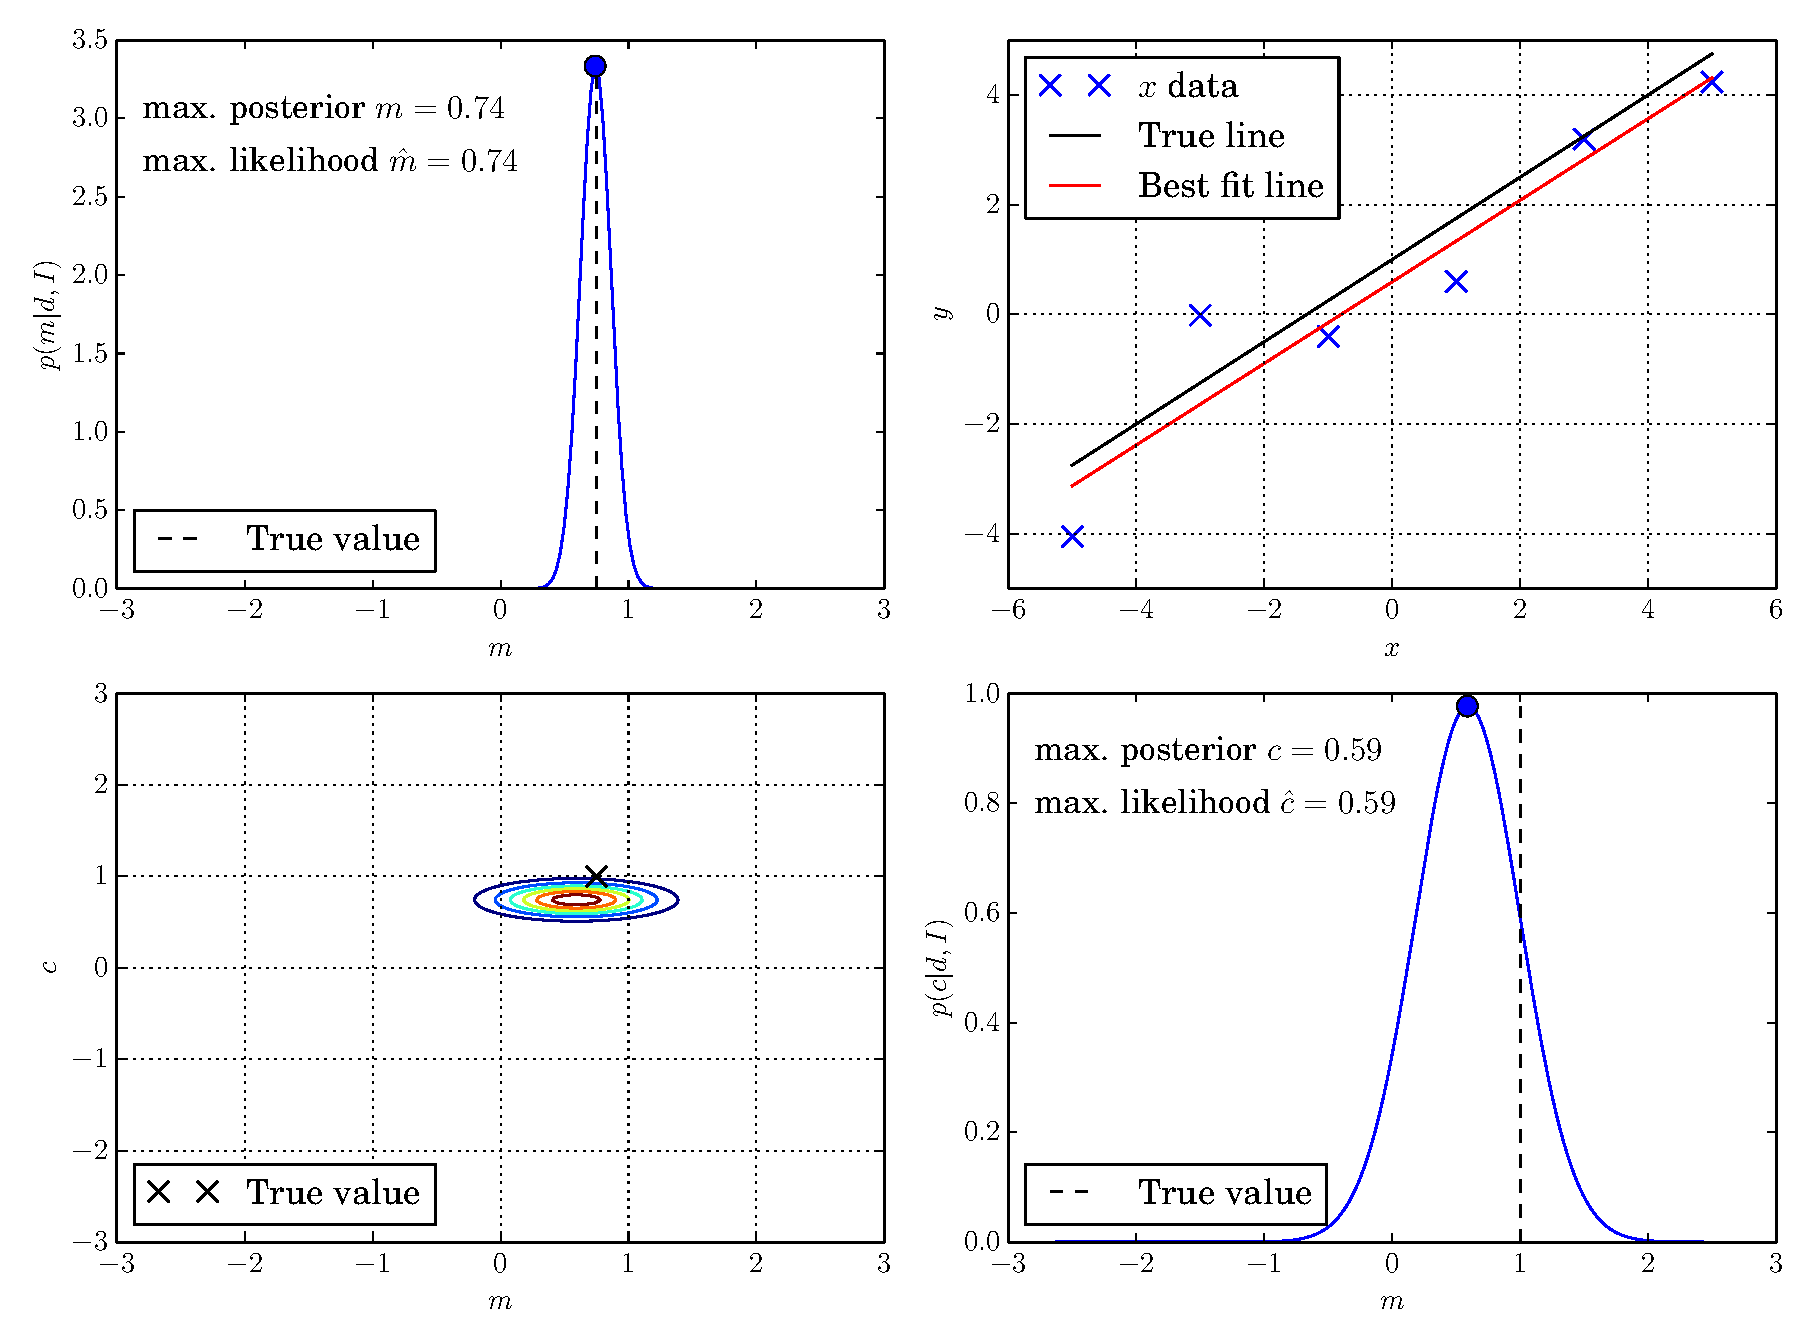
\includegraphics[keepaspectratio,width=\textwidth,height=210pt]{figures/bayesian_line_fitting.pdf}
\label{bayesian_line_fitting}
\end{figure}

\end{frame}

\begin{frame}

\frametitle{Example: fitting a line}
\label{example:fittingaline}

In the above example, in practice, when $p(m,c|I) = \text{constant}$ and $\sigma_i = \sigma$ are constant, we can just calculate the posterior\footnote{We generally work in natural logarithm space due to numerical precision issues.} over a grid in $m$ and $c$
\[
\ell(m_{i_m},c_{i_c}) = \ln{p(m_{i_m},c_{i_c}|d,I)} = -\sum_{i=1}^n\frac{[d_i-(m_{i_m} x_i + c_{i_c})]^2}{2\sigma^2}
\]
and get the marginal posteriors through numerical integration, e.g.
\[
p(m_{i_m}|d,I) \propto \sum_{i_c}^{n_c} \exp{\left(\ell(m_{i_m},c_{i_c}) - \text{max}\ell(m,c)\right)} \Delta c
\]
where $\Delta c$ are the grid step sizes in $c$ (or you could use the trapezium rule for more acurracy).

\end{frame}

\begin{frame}

\frametitle{Example: fitting a line}
\label{example:fittingaline}

What if we don't know $\sigma$?

In this case we can treat $\sigma$ as another unknown variable and marginalise over it, e.g.
\[
p(m,c|d,I) = p(m,c|I) \int_0^{\infty} p(d|m,c,\sigma,I)p(\sigma|I) {\rm d}\sigma
\]
If the likelihood is Gaussian and we assume a flat prior on all parameters, e.g.
\[
p(\sigma|I) = \begin{cases}C, \sigma > 0 \\ 0, \sigma \le 0\end{cases}
\]
Then we have
\[
p(m,c|d,I) \propto \int_0^{\infty} \sigma^{-n} \exp{\left(-\sum_{i=1}^n\frac{[d_i-(m x_i + c)]^2}{2\sigma^2}\right)} {\rm d}\sigma
\]

\end{frame}

\begin{frame}

\frametitle{Example: fitting a line}
\label{example:fittingaline}

This integral is analytic, and through some substitution (see e.g. Chap. 3 of Sivia~\citep{Sivia}), becomes
\[
p(m,c|d,I) \propto \left( \sum_{i=1}^n [d_i-(m x_i + c)]^2 \right)^{-(n-1)/2}
\]
This is essentially a \emph{Student's $t$-distribution} with $\nu = (n-2)$ degrees of freedom.

Note: if we were instead to use a prior on $\sigma$ of $p(\sigma|I) \propto 1/\sigma$ it would
lead to a Student's $t$-distribution with $\nu = n-1$ degrees of freedom.

\end{frame}

\begin{frame}

\frametitle{Example: fitting a line}
\label{example:fittingaline}

\begin{figure}[htbp]
\centering
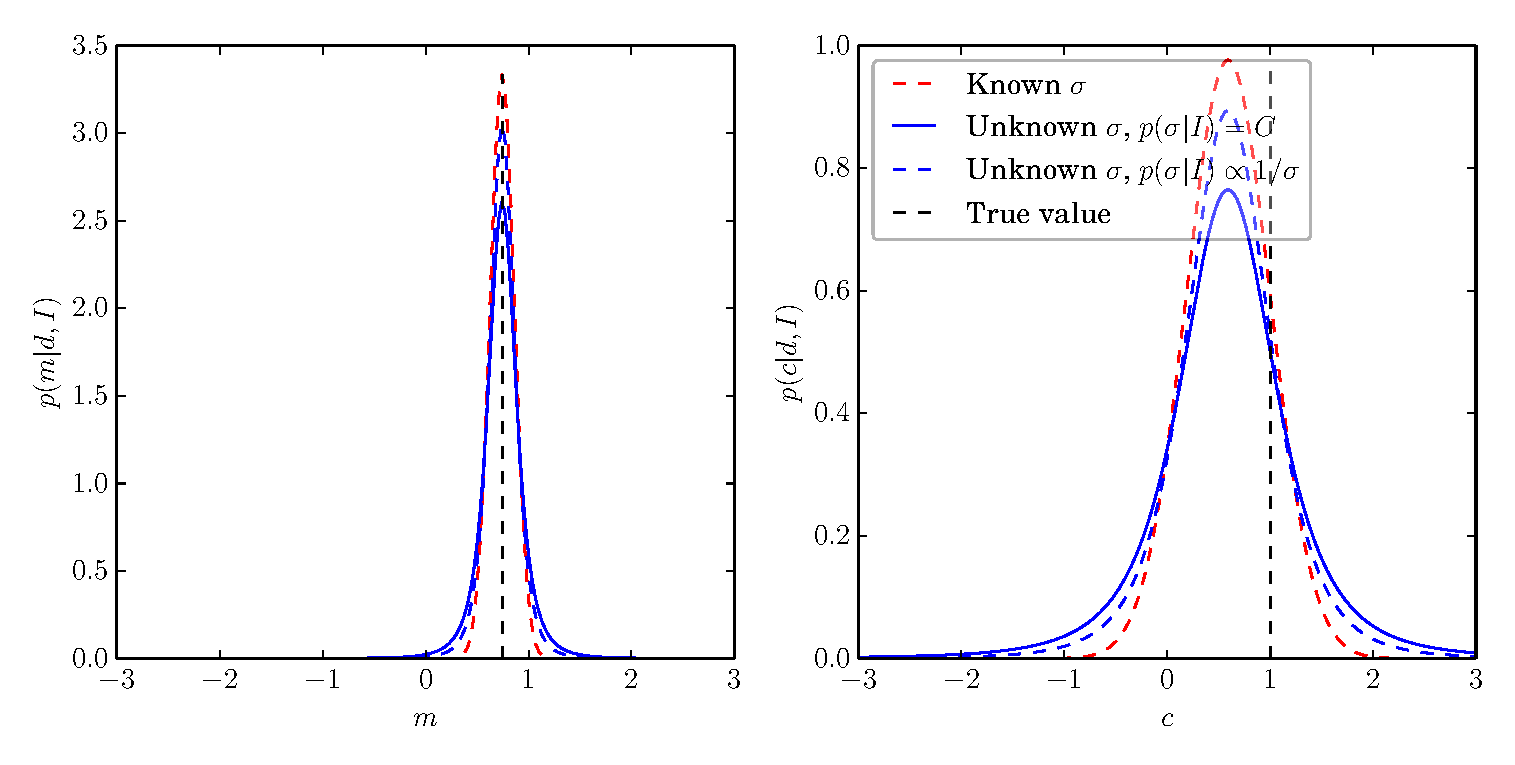
\includegraphics[keepaspectratio,width=\textwidth,height=210pt]{figures/bayesian_line_fitting_2.pdf}
\label{bayesian_line_fitting_2}
\end{figure}

\end{frame}

\begin{frame}

\frametitle{Example: spectral line estimation}
\label{example:spectrallineestimation}

We take a simple example: \emph{finding the frequency of a sinusoid in noisy data}\footnote{Performing spectral estimation in a Bayesian sense is discussed in great detail in Bretthorst~\citep{Bretthorst}}. We can model the signal as
\[
y(t_i) = C\cos{(\omega t_i + \phi)} = \redub{A}_{C\cos{\phi}}\cos{(\omega t_i)} + \redub{B}_{-C\sin{\phi}}\sin{(\omega t_i)}
\]
where $\omega = 2\pi f$ is the angular frequency and $A$ and $B$ are two unknown amplitudes (accounting for an
unknown amplitude and initial phase of the signal).

A standard way to do this is performing a Fourier transform, and creating e.g. a power spectrum.

\end{frame}

\begin{frame}

\frametitle{Example: spectral line estimation}
\label{example:spectrallineestimation}

In this case we have four unknowns: $A$, $B$, $\omega$, and $\sigma$ (we assume unknown noise) but we are only interested in $\omega$, so given some data $d$,
we want to calculate
\[
p(\omega|d,I) \propto \int_{-\infty}^{\infty}\int_{-\infty}^{\infty}\int_{0}^{\infty} p(d|\omega,A,B,\sigma,I) p(\omega,A,B,\sigma|I) {\rm d}A {\rm d}B {\rm d}\sigma
\]
where, assuming Gaussian noise on the data, the likelihood is given by
\begin{align*}
p(d|\omega,A,B,\sigma,I) &\propto \sigma^{-n}\exp{\left(-\sum_{i=1}^n\frac{[d_i-y(t_i)]^2}{2\sigma^2}\right)} \\
&= \sigma^{-n}\exp{\left(-\frac{nQ}{2\sigma^2}\right)}.
\end{align*}

\end{frame}

\begin{frame}

\frametitle{Example: spectral line estimation}
\label{example:spectrallineestimation}

The quadratic form is given by
\[
Q = \redub{\bar{d^2}}_{\mathclap{\frac{1}{n}\sum_{i=1}^n d_i^2}} - \frac{2}{n}[ A\redob{R(\omega)}^{\mathclap{\sum_{i=1}^nd_i\cos{\omega t_i}}} + B\redub{I(\omega)}_{\mathclap{\sum_{i=1}^nd_i\sin{\omega t_i}}}] + \frac{1}{2}(A^2 + B^2)
\]
where the following approximations have been made
\[
\sum_{i=1}^n \cos{}^2\omega t_i \approx  \sum_{i=1}^n \sin{}^2\omega t_i \approx \frac{n}{2} \text{ and } \sum_{i=1}^n \sin{\omega t_i}\cos{\omega t_i} \approx 0,
\]
which are valid if $n \gg 1$ and the data doesn't contain very low frequencies.

\end{frame}

\begin{frame}

\frametitle{Example: spectral line estimation}
\label{example:spectrallineestimation}

Assuming flat priors on $A$ and $B$ we can analytically integrate them (e.g. with \texttt{Mathematica}), giving
\[
p(\omega|d,I) \propto \int_0^{\infty} \sigma^{-n+2}\exp{\left[-\frac{n}{2\sigma^2}\{\bar{d^2} - 2(R^2 + I^2)/n\} \right]}p(\sigma|I).
\]
If we take $p(\sigma|I) \propto 1/\sigma$, the the intergal over $\sigma$ is again analytic, again leading to the Student's $t$-distribution, with $\nu = (n-3)$ degrees of freedom
\[
p(\omega|d,I) \propto \left[1 - \frac{2(R^2 + I^2)}{n\bar{d^2}}\right]^{-(n-2)/2}
\]
Or, if we know $\sigma$ we would just have
\[
p(\omega|d,I) \propto \exp{\left(\frac{R^2 + I^2}{\sigma^2}\right)}
\]

\end{frame}

\begin{frame}

\frametitle{Example: spectral line estimation}
\label{example:spectrallineestimation}

We can compare this with a standard power spectrum:

\begin{figure}[htbp]
\centering
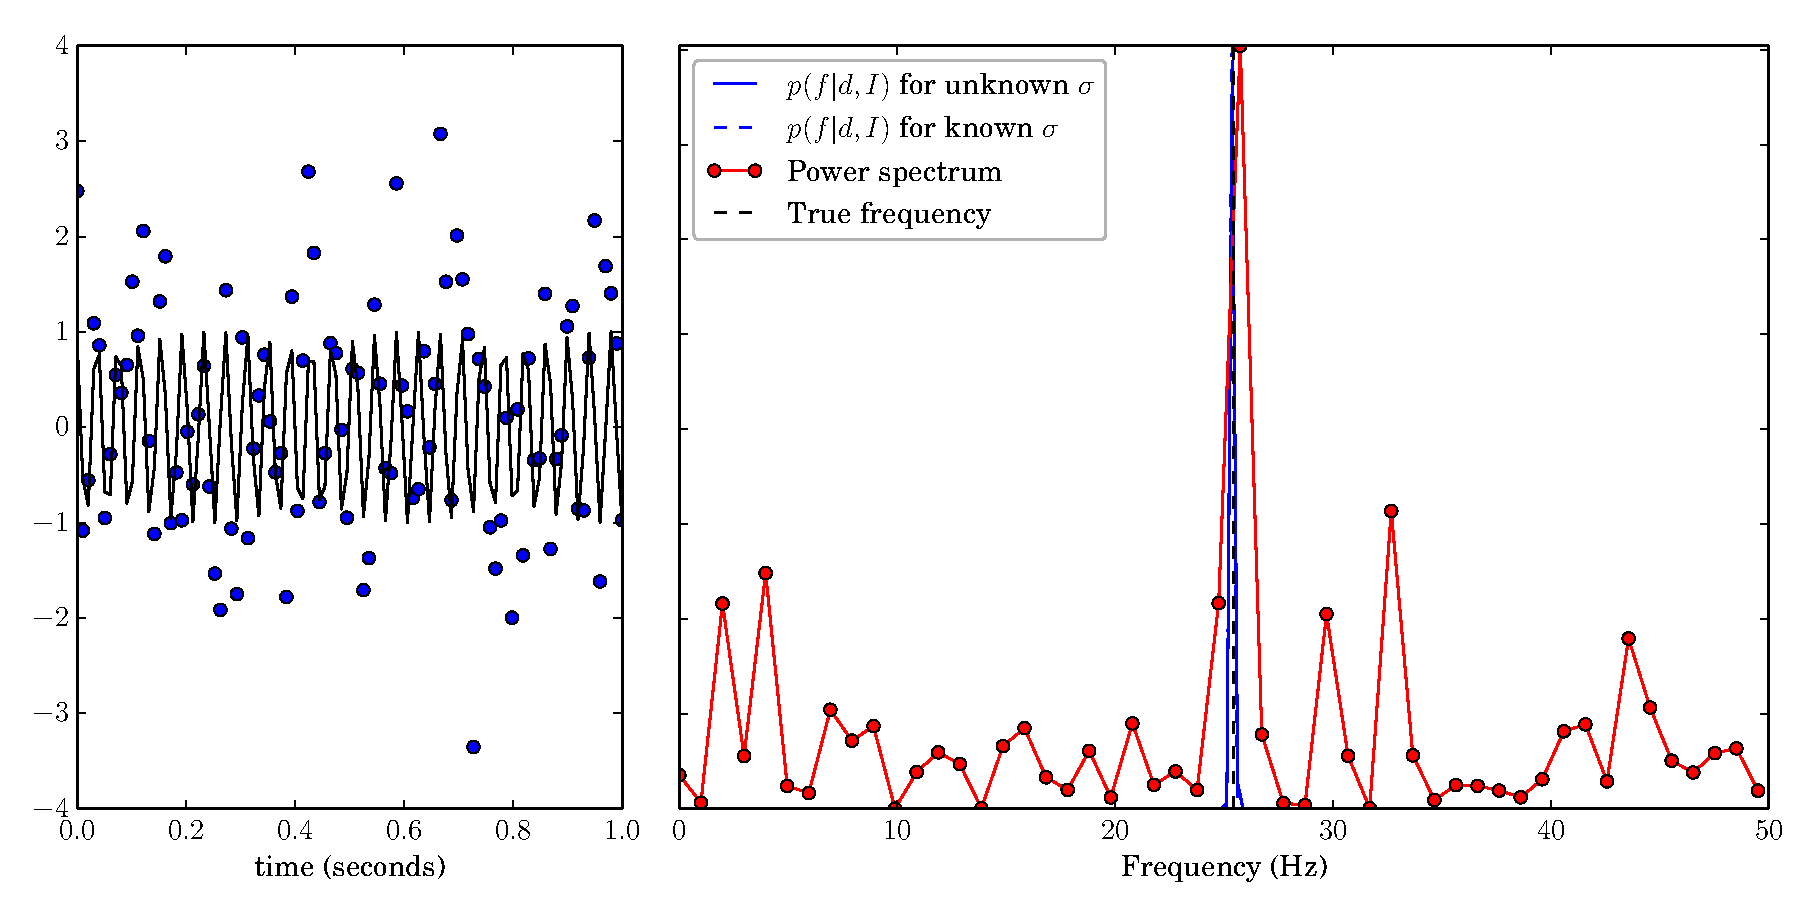
\includegraphics[keepaspectratio,width=\textwidth,height=200pt]{figures/spectral_estimation.pdf}
\label{spectral_estimation}
\end{figure}

\end{frame}

\begin{frame}

\frametitle{Bayesian parameter estimation}
\label{bayesianparameterestimation}

From these examples we see that we could apply it to any model with any number of parameters.
However, for these examples we have either had an intrinsically small number of parameters, or
been able to analytically marginalise over them. This makes it easy to compute posteriors on a
grid.

As the number of parameters increases the number of grid points would have to also increase to keep
a decent resolution on each parameter, e.g. a posterior evaluated on a grid of 10 points for each of
$M$ parameters, would required $10^M$ evaluations. This can be prohibitive and we may need to use
methods like \emph{Markov chain Monte Carlo}.

\end{frame}

\begin{frame}

\frametitle{Defining probabilities: choice of prior}
\label{definingprobabilities:choiceofprior}

Probability (even with frequentist methods) \emph{is} subjective and depends on the available information.
\begin{center}
But: {\color{red}Subjective $\ne$ Arbitrary}
\end{center}
Bernoulli (1713) set out the `Principle of insufficient reason' and Keynes (1921) the `Principle of indifference':

\emph{Given the \textbf{same} background information, two observers should assign the \textbf{same} probabilities}

E.g. for a die we should all agree that given it has 6 faces (and no contrary information)
we should assign the proposition $X_i \equiv \text{``the face on top has }i\text{ dots''}$ $p(X_i|I) = \frac{1}{6}$ for all $i$

\end{frame}

\begin{frame}

\frametitle{Defining probabilities: choice of prior}
\label{definingprobabilities:choiceofprior}

Can we justify this more fundamentally?

In the case of the die, we could have assigned the proposition $X_i \equiv \text{``the face on top has }7-i\text{ dots''}$, but we \emph{should still have} $p(X_i|I) = \frac{1}{6}$ for all $i$

If we extend this to the continuum case, setting $x$ to be a \textbf{location parameter}\footnote{E.g. a parameter that can be defined over positive and negative values.}, the `principle of indifference'
means we should have
\[
 p(x|I){\rm d}x = p(x+\Delta|I){\rm d}(x+\Delta)
\]
where $\Delta$ is a constant. Since ${\rm d}(x+\Delta)/{\rm d}x = 1$, we must have
\[
\boxed{p(x|I) = \text{constant}}
\]

\end{frame}

\begin{frame}

\frametitle{Defining probabilities: choice of prior}
\label{definingprobabilities:choiceofprior}

Similarly, if we let $s$ be a \textbf{scale parameter}\footnote{E.g. a parameter defined as only having positive values and indifferent to a change in units.}, the `principle of indifference'
means we should have
\[
p(s|I){\rm d}s = p(\beta s|I){\rm d}(\beta s)
\]
where $\beta$ is a positive constant (e.g. a conversion factor between two sets of units).
Since ${\rm d}(\beta s)/{\rm d}s = \beta$ we must have
\[
\frac{p(s|I)}{p(\beta s|I)} = \beta,
\]
so,
\[
\redub{\boxed{p(s|I) \propto \frac{1}{s}}}_{\mathclap{\text{Jeffreys' prior}}}
\]

\end{frame}

\begin{frame}

\frametitle{Defining probabilities: Jeffreys' prior}
\label{definingprobabilities:jeffreysprior}

A Jeffreys' prior represents complete ignorance about the value of a scale parameter (we used this for the
prior in $\sigma$ in the spectral estimation case).

It is equivalent to a uniform pdf for the logarithm of $s$
\[
p(\log{s}|I) {\rm d}s = \text{constant}.
\]
If an upper and lower range on $s$ were known then we have
\[
p(s|I) = \frac{1}{s\ln{(s_{\rm max}/s_{\rm min})}}
\]

\end{frame}

\begin{frame}

\frametitle{Defining probabilities: Jeffreys' prior}
\label{definingprobabilities:jeffreysprior}

This form of the Jeffreys' prior, $p(L|I) \propto 1/L$, is just the special case of a more general result. If
we had a likelihood with parameters $\vec{\theta}$ then the \textbf{Jeffreys' prior} is a non-informative prior
defined as
\[
p(\vec{\theta}) \propto [|I(\vec{\theta}|]^{1/2}.
\]
In this $I(\vec{\theta})$ is the \textbf{Fisher Information} defined as
\[
I(\vec{\theta})_{i,j} = E\left[\frac{\partial \ln{L(\vec{\theta})}}{\partial \theta_i}
\frac{\partial \ln{L(\vec{\theta})}}{\partial \theta_j}\right]
\]

This prior is \textbf{invariant} under \textbf{any} re-parameterisation of $\vec{\theta}$ (i.e. scalings or
translations).

\end{frame}

\begin{frame}

\frametitle{Defining probabilities: Maximum entropy}
\label{definingprobabilities:maximumentropy}

How do we deal with situation where we know some constraints?

E.g. suppose a six-sided die was rolled many times and the average results was 4.5
then what probability should be assign the various outcomes $p(X_i|I)$? This constraint
information
\[
\sum_{i=1}^6 i p(X_i|I) = 4.5
\]
is \textbf{testable information}. A way to assign $p(X_i|I)$ is to \textbf{maximise the entropy}
\[
S = -\sum_{i=1}^6 p(X_i|I) \ln{p(X_i|I)}
\]
given the above constraint and the condition $\sum_i p(X_i|I) = 1$.

\end{frame}

\begin{frame}

\frametitle{Defining probabilities: Maximum entropy}
\label{definingprobabilities:maximumentropy}

\begin{columns}
     \begin{column}{0.5\textwidth}

$p(X_i|I)$ can be solved for in $\frac{{\rm d}S}{{\rm d}X} = 0$, using e.g. \emph{Lagrange Multipliers}, and yields:
\end{column}
\begin{column}{0.5\textwidth}
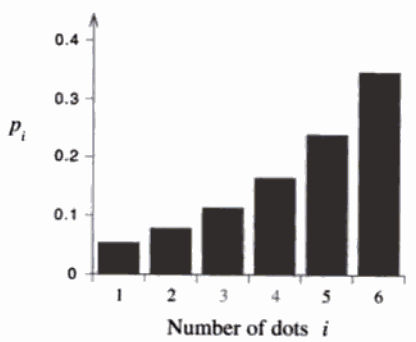
\includegraphics[keepaspectratio,width=\textwidth,height=100pt]{figures/maxent.png}
\end{column}
\end{columns}

The MaxEnt approach can be justified using a varirty of approaches, e.g.

\begin{itemize}
\item Independence arguments (see e.g. \href{http://cmm.cit.nih.gov/maxent/kangaroo.html}{\emph{the kangeroo problem}}\footnote{\href{http://cmm.cit.nih.gov/maxent/kangaroo.html}{http:/\slash cmm.cit.nih.gov\slash maxent\slash kangaroo.html}})

\end{itemize}

\end{frame}

\begin{frame}

\frametitle{Defining probabilities: common pdfs}
\label{definingprobabilities:commonpdfs}

MaxEnt can be used to yield many common pdfs.

If we know the expected value, $\mu$, of a continuous physical quantity, then using MaxEnt we find
\[
\redub{p(x|\mu,I) = \frac{1}{\mu}\exp{\left(-\frac{x}{\mu}\right)}}_{\mathclap{\text{Exponential distribution}}}
\]
or, for a \emph{discrete} physical quantity $N$ we find
\[
\redub{p(N|\mu,I) = -\frac{\mu^N e^{-\mu}}{N!}}_{\mathclap{\text{Poisson distribution}}}
\]

\end{frame}

\begin{frame}

\frametitle{Defining probabilities: common pdfs}
\label{definingprobabilities:commonpdfs}

If we know the expected value, $\mu$, and variance, $\sigma^2$, of a continuous physical quantity, then MaxEnt shows
\[
\redub{p(x|\mu,\sigma,I) = \frac{1}{\sqrt{2\pi\sigma^2}}\exp{\left(-\frac{(x-\mu)^2}{2\sigma^2} \right)}}_{\mathclap{\text{Normal distribution}}}
\]

This justifies the relevance of common pdfs. E.g. if we know $\mu$ and $\sigma^2$ then our least informative
(so generally most conservative) pdf is the normal, which is often why it is so ubiquitous as a likelihood function. 

However, if we have other information then we could improve our posteriors by using that information to
assign a more relevant pdf.

\end{frame}

\begin{frame}

\frametitle{Bayesian hypothesis testing}
\label{bayesianhypothesistesting}

Unlike frequentist methods that require assessing some statistic to compare two hypotheses in
Bayesian hypothesis testing (or \textbf{model selection}) we just directly calculate the probability
of each hypothesis and compare them. E.g., if we have two hypotheses $H_1$ and $H_2$ (these could
be any propositions), then
\begin{align*}
\text{if } \frac{p(H_1|I)}{p(H_2|I)} > 1 & \text{ then } H_1 \text{ is favoured}, \\
\text{if } \frac{p(H_1|I)}{p(H_2|I)} < 1 & \text{ then } H_2 \text{ is favoured}, \\
\end{align*}
This is a \textbf{Bayesian odds ratio}, but how do we compute it?

\end{frame}

\begin{frame}

\frametitle{Bayesian hypothesis testing}
\label{bayesianhypothesistesting}

Suppose our two hypothesis represent two models defined by parameters $\vec{\theta}_1$ and
$\vec{\theta}_2$, and we want to test which model if favoured given a set of data $d$. We can
just apply Bayes' theorem
\[
\mathcal{O}_{12} = \frac{p(H_1|d,I)}{p(H_2|d,I)} = \frac{\left( \frac{p(d|H_1,I)p(H_1|I)}{\cancel{p(d|I)}} \right)}
{\left( \frac{p(d|H_2,I)p(H_2|I)}{\cancel{p(d|I)}} \right)} = \redub{\frac{p(d|H_1,I)}{p(d|H_2,I)}}_{\mathclap{\text{Bayes factor}}} \redub{\frac{p(H_1|I)}{p(H_2|I)}}_{\mathclap{\text{Prior odds}}}
\]

\begin{itemize}
\item \textbf{Prior odds} - our prior knowledge about each model, often set to $1$ (i.e. no preference for either model)

\item \textbf{Bayes factor} - ratio of \textbf{evidences}, or \textbf{marginal likelihoods}, for each model.

\end{itemize}

\end{frame}

\begin{frame}

\frametitle{Bayesian hypothesis testing}
\label{bayesianhypothesistesting}

Note $p(H|d,I)$ is a \emph{probability density function} not a probability, so we can't interpret particular values
of it (e.g. $p(H_1|d,I)$) on their own.

Unless we can define the entire hypothesis space, so probabilities are given by e.g.
\[
\text{prob}(H_1 \le H \le H_2|d,I) = \int_{H_1}^{H_2} p(H|d,I) {\rm d}H
\]
we can only compare $p(H|d,I)$ for distinct different hypotheses
\[
\frac{p(H_1|d,I)}{p(H_2|d,I)}.
\]
But, in general, this is all we want to do.

\end{frame}

\begin{frame}

\frametitle{Bayesian hypothesis testing}
\label{bayesianhypothesistesting}

How do we calculate the \textbf{evidence}? For model $1$ we have a posterior on $\vec{\theta}_1$ defined as
\[
p(\vec{\theta}_1|d,H_1,I) = \frac{p(\vec{\theta}_1|d,H_1,I)p(\vec{\theta}_1|H_1,I)}{\redub{p(d|H_1,I)}_{\mathclap{\text{evidence}}}}
\]
The \emph{evidence}, $Z$, is the normalisation constant that makes $\int p(\vec{\theta}_1|d,H_1,I) {\rm d}\vec{\theta}_1 = 1$, so
\[
Z_1 = p(d|H_1,I) = \int_{\vec{\theta}_1}p(\vec{\theta}_1|d,H_1,I)p(\vec{\theta}_1|H_1,I) {\rm d} \vec{\theta}_1
\]

\end{frame}

\begin{frame}

\frametitle{Bayesian hypothesis testing}
\label{bayesianhypothesistesting}

If this integral is analytic then the \emph{evidence} is easy to calculate, or \emph{if} $\vec{\theta}$
contains only a few (say less than 6) parameters, then it is relatively easy to calculate
numerically over a parameter space grid. But, as with parameter estimation, over high
dimensional models it becomes a computational challenge to compute.

We may need to use integral approximations, or e.g. \emph{nested sampling} ~\citep{Skilling}.

\end{frame}

\begin{frame}

\frametitle{Bayesian hypothesis testing: example}
\label{bayesianhypothesistesting:example}

\begin{columns}
\begin{column}{0.5\textwidth}

Let's take two hypotheses:

\begin{itemize}
\item $H_1$ - the data contains a line defined by an unknown gradient $m$ and y-intercept $c$

\item $H_2$ - the data is consistent with Gaussian random noise with zero mean and unit variance

\end{itemize}

We will assume that the variance, $\sigma^2=1$, of the noise in the data is known. So, we
need to find the evidence for each hypothesis.
\end{column}
\begin{column}{0.5\textwidth}
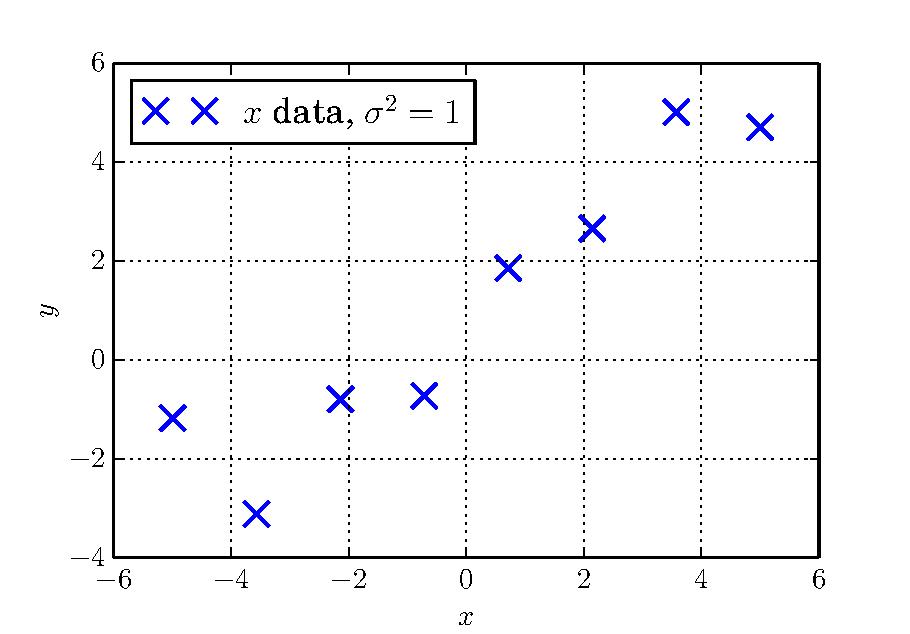
\includegraphics[keepaspectratio,width=\textwidth,height=210pt]{figures/linear_data_2.pdf}
\end{column}
\end{columns}

\end{frame}

\begin{frame}

\frametitle{Bayesian hypothesis testing: example}
\label{bayesianhypothesistesting:example}

We first need to assign priors on $m$ and $c$. Just looking at the data we can see that
reasonable ranges are:

\begin{itemize}
\item $0 \le m \le 5$ (i.e. the slope isn't negative, or very steep)

\item $-2 \le c \le 4$

\end{itemize}

so,
\[
p(m|H_1,I) = \begin{cases} 1/(5-0) = 0.2, \text{ if } 0 \le m \le 5 \\ 0, \text{ otherwise}\end{cases}
\text{ and }
\]
\[
p(c|H_1,I) = \begin{cases} 1/(4--2) = 0.167, \text{ if } -2 \le m \le 4 \\ 0, \text{ otherwise}\end{cases}
\]
Later we will see how changes in these prior ranges effect things.

\end{frame}

\begin{frame}

\frametitle{Bayesian hypothesis testing: example}
\label{bayesianhypothesistesting:example}

So, we now need to compute
\begin{align*}
Z_1 &= \int_{m=0}^5 \int_{c=-2}^4 p(m|H_1,I)p(c|H_1,I)p(d|m,c,H_1,I) {\rm d}m{\rm d}c,\\
&= \frac{0.033}{(2\pi \sigma^2)^{n/2}} \int_{m=0}^5 \int_{c=-2}^4 \exp{\left(-\sum_{i=1}^n\frac{(d_i - (mx_i+c))^2}{2\sigma^2} \right)} {\rm d}m{\rm d}c
\end{align*}
This integral is analytical (or at least involves erf) so can be computed easily. For our given data, with
$n=8$ and $\sigma^2 = 1$, we find (working in natural logarithms)
\[
\ln{Z_1} = -16.0. 
\]

\end{frame}

\begin{frame}

\frametitle{Bayesian hypothesis testing: example}
\label{bayesianhypothesistesting:example}

We now need the evidence that the data just consists of Gaussian noise with zero mean and variance $\sigma^2 = 1$, so we have
\begin{align*}
Z_2 &= \frac{1}{(2\pi \sigma^2)^{n/2}} \exp{\left(-\sum_{i=1}^n\frac{d_i^2}{2\sigma^2} \right)}, \\
\ln{Z_2} &= -42.4.
\end{align*}
So, in this case the odds ratio for the two models is:
\[
\mathcal{O}_{12} = \exp{(\ln{Z_1}-\ln{Z_2})} = \exp{(-16.0 + 42.4)} = 2.8\times 10^{11}!
\]
\emph{The data is definitely better explained by a line than Gaussian noise.} 

\end{frame}

\begin{frame}

\frametitle{Bayesian hypothesis testing: example}
\label{bayesianhypothesistesting:example}

What happens in the above case if we say that we already know that $c = 1$ (call this
hypothesis $H_3$)?

We can again calculate the evidence in this case as
\begin{align*}
Z_3 &= \int_{m=0}^5 p(m|H_3,I)p(d|m,c,H_3,I) {\rm d}m,\\
&= \frac{0.2}{(2\pi \sigma^2)^{n/2}} \int_{m=0}^5 \exp{\left(-\sum_{i=1}^n\frac{(d_i - (mx_i+1))^2}{2\sigma^2} \right)} {\rm d}m \\
\ln{Z_3} &= -14.1.
\end{align*}
We see $H_3$ is favoured over $H_1$ by a factor of $e^{(-14.1+16.0)} = 6.7$. But, $H_3$ is just
a subhypothesis included within $H_1$, so why is it favoured?

\end{frame}

\begin{frame}

\frametitle{Bayesian hypothesis testing: Occam factor}
\label{bayesianhypothesistesting:occamfactor}

This is an example of the \textbf{`Occam factor'} that is automatically incorporated in Bayesian
model selection.

\begin{columns}
     \begin{column}{0.6\textwidth}
\begin{center}
{\color{red} Occam's razor}: ``\textbf{Plurality should not be posited without necessity}''
\end{center}
\end{column}
\begin{column}{0.4\textwidth}

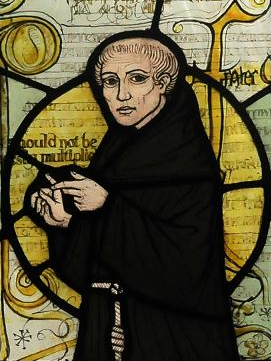
\includegraphics[keepaspectratio,width=\textwidth,height=100pt]{figures/Ockham.png}
\end{column}
\end{columns}
This principle means that more complicated models (i.e. with more parameters or larger parameter
ranges) should be penalised \emph{if} they do not contribute enough additional evidence.

\end{frame}

\begin{frame}

\frametitle{Bayesian hypothesis testing: Occam factor}
\label{bayesianhypothesistesting:occamfactor}

\begin{columns}
     \begin{column}{0.525\textwidth}

We can also see Occam's razor in action if we again take hypothesis $H_3$, but also have $H_4$ with double
the prior range to $p(-2.5 \le m \le 7.5|H_4,I) = 0.1$. Here $H_3$ is twice as probable as $H_4$: the likelihood is entirely within $p(m|H_3,I)$, so expanding
the range adds no extra information.

If the prior were hugely expanded the model containing a line would still highly favoured over
Gaussian noise.

\end{column}
\begin{column}{0.475\textwidth}

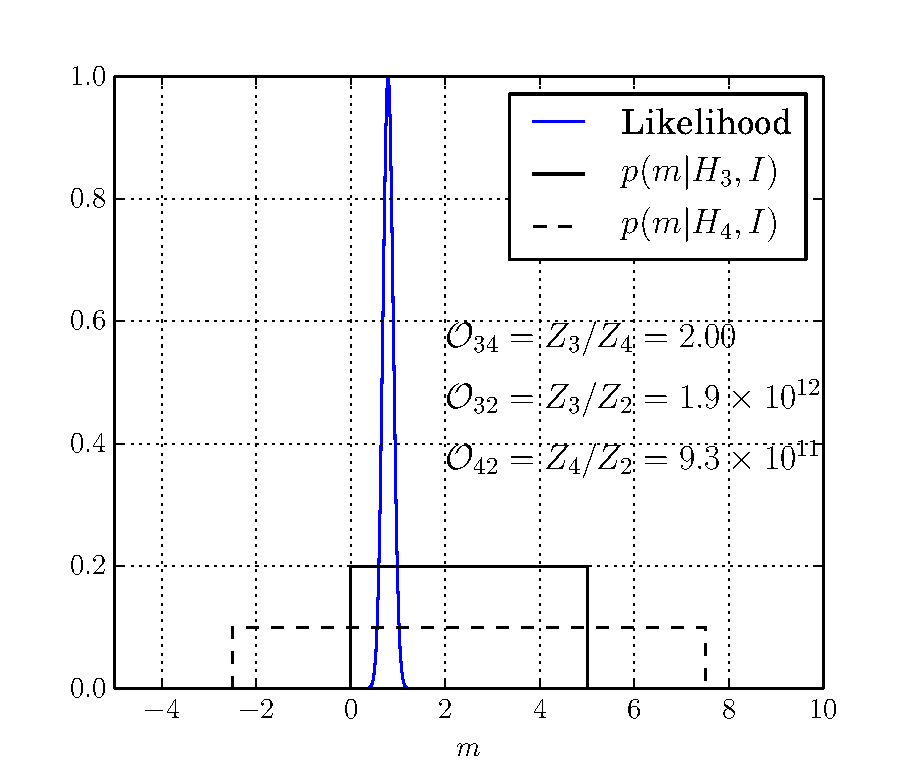
\includegraphics[keepaspectratio,width=\textwidth,height=180pt]{figures/occam_factor.pdf}
\end{column}
\end{columns}

\end{frame}

\begin{frame}

\frametitle{Bayesian hypothesis testing}
\label{bayesianhypothesistesting}

We also can make statements about compound hypotheses e.g.
\[
\mathcal{O}_{H_1\text{ \textbf{and} }H_2 \text{ vs. }H_3} = \frac{p(H_1|d,I)p(H_2|d,I)}{p(H_3|d,I)}
\]
or,
\[
\mathcal{O}_{H_1\text{ \textbf{or} }H_2 \text{ vs. }H_3} = \frac{p(H_1|d,I) + p(H_2|d,I)}{p(H_3|d,I)}.
\]

Or, we could compare multiple hypotheses, such as data being described by a polynomial with different numbers
of coefficients, $N$, to see which provides the best fit.

\end{frame}

\begin{frame}

\frametitle{Bayesian hypothesis testing: approximations}
\label{bayesianhypothesistesting:approximations}

Calculating the evidence can be computationally costly, so an approximate way to calculate the Bayes factor is
the \textbf{Bayesian Information Criterion} (BIC) ~\citep{Schwarz}
\[
\text{BIC} = 2\ln{L_{\rm max}} + k\ln{n}
\]
where $L_{\rm max}$ is the maximum likelihood, $k$ is the number of parameters in model, and $n$ is
the number of data points.

We can (roughly) say:

\begin{itemize}
\item If $\text{BIC}_1 - \text{BIC}_2 > 2$ there is positive evidence for model 1

\item If $\text{BIC}_1 - \text{BIC}_2 > 6$ there is \emph{strong} evidence for model 1

\end{itemize}

A better approximation to the Bayes factor is the \textbf{Laplace approximation}, which assumes a multivariate Gaussian posterior (see e.g. ~\citep{Trotta}).

\end{frame}

\begin{frame}

\frametitle{Parameter estimation: the Gaussian approximation}
\label{parameterestimation:thegaussianapproximation}

Posteriors can sometimes be approximated by a Gaussian distribution. This can be justified
through a maximum likelihood type approach (which in turn provides a Bayesian foundation to
frequentist maximum likelihood estimators).

The maximum posterior is found when
\[
\frac{\partial p(\theta|d,I)}{\partial \theta}\Big|_{\theta=\theta_0} = 0
\]
Equivalently we can define $\ell = \ln{p(\theta|d,I)}$ and compute $\frac{\partial \ell}{\partial \theta}\big|_{\theta=\theta_0} = 0$. If we Taylor expand $\ell(\theta)$ around $\theta=\theta_0$ then
\[
\ell(\theta) = \ell(\theta_0) + \redub{\cancel{\frac{\partial \ell}{\partial \theta}\Bigg|_{\theta=\theta_0}}}_{\mathclap{\text{=0}}}(\theta-\theta_0) + \frac{1}{2}\frac{\partial^2 \ell}{\partial \theta^2}\Bigg|_{\theta=\theta_0}(\theta-\theta_0)^2 + \ldots
\]

\end{frame}

\begin{frame}

\frametitle{Parameter estimation: the Gaussian approximation}
\label{parameterestimation:thegaussianapproximation}

So, the posterior is given by
\[
p(\theta|d,I) = \exp{[\ell(\theta)]}
\]
and neglecting higher order terms in $\ell(\theta)$ (the \textbf{Gaussian approximation}) gives
\[
p(\theta|d,I) \propto \exp{\left(-\frac{A}{2}(\theta - \theta_0)^2\right)},
\]
where
\[
A = -\frac{\partial^2 \ell}{\partial \theta^2}\Bigg|_{\theta=\theta_0}
\]
This is equivalent to a \textbf{normal} distribution with $\sigma^{-2} = A$.

In these cases we can summarise inference from the posterior with: $\theta = \theta_0 \pm \sigma$.

\end{frame}

\begin{frame}

\frametitle{The Gaussian approximation (2D)}
\label{thegaussianapproximation2d}

For two parameters we have a posterior
\[
p(\theta_1,\theta_2|d,I) \propto p(d|\theta_1,\theta_2,I) \times p(\theta_1,\theta_2|I)
\]
and the `best' estimator at the posterior maximum is
\[
\frac{\partial p(\theta_1,\theta_2|d,I)}{\partial \theta_j}\Bigg|_{\theta_j=\theta_{0,j}} = 0
\]
Compute $\frac{\partial \ell}{\partial \theta_j}\big|_{\theta_j=\theta_{0,j}}$ where $\ell = \ln{p(\theta_1,\theta_2|d,I)}$.

\end{frame}

\begin{frame}

\frametitle{The Gaussian approximation (2D)}
\label{thegaussianapproximation2d}

We again Taylor expand $\ell(\theta_1,\theta_2)$ about $\theta_{0,j}$ giving
\[
\begin{array}{l}
\ell(\theta_1,\theta_2) = \ell(\theta_{0,1},\theta_{0,2}) + \cancel{\frac{\partial \ell}{\partial \theta_1}\Big|_{\theta_1=\theta_{0,1}}}(\theta_1-\theta_{0,1}) + \\
\cancel{\frac{\partial \ell}{\partial \theta_2}\Big|_{\theta_2=\theta_{0,2}}}(\theta_2-\theta_{0,2}) + 
\frac{1}{2}\Bigg[ \frac{\partial^2 \ell}{\partial \theta^2_1}\Big|_{\theta_1=\theta_{0,1}}(\theta_1-\theta_{0,1})^2 + 
\\
\frac{\partial^2 \ell}{\partial \theta^2_2}\Big|_{\theta_2=\theta_{0,2}}(\theta_2-\theta_{0,2})^2 +
 2\frac{\partial^2 \ell}{\partial \theta_1 \partial \theta_2}\Big|_{\theta_j=\theta_{0,j}}(\theta_1-\theta_{0,1})(\theta_2 - \theta_{0,2})\Bigg]
\end{array}
\]
so, the Gaussian approximation, is
\[
p(\theta_1,\theta_2|d,I) \propto \exp{[\ell(\theta_1,\theta_2)]} \propto \exp{\left[-\frac{1}{2}Q\right]}
\]

\end{frame}

\begin{frame}

\frametitle{The Gaussian approximation (2D)}
\label{thegaussianapproximation2d}

We have put this in matrix form to have the quadratic form
\[
Q = (\theta_1-\theta_{0,1}, \theta_2-\theta_{0,2})\left[ 
\begin{array}{cc}
A & C \\
C & B
\end{array}\right]\left( \begin{array}{c}
\theta_1-\theta_{0,1} \\
\theta_2-\theta_{0,2}
\end{array}\right),
\]
where
\[
A = \frac{\partial^2 \ell}{\partial \theta^2_1}\Big|_{\theta_1=\theta_{0,1}}, 
B = \frac{\partial^2 \ell}{\partial \theta^2_2}\Big|_{\theta_2=\theta_{0,2}}, \text{ and }
C = \frac{\partial^2 \ell}{\partial \theta_1 \partial \theta_2}\Big|_{\theta_j=\theta_{0,j}}
\]
This is the \textbf{bivariate normal distribution} with covariance matrix defined using $C$.

This can be generalised to any number of parameters
\[
\sigma_{i,j}^2 = \langle(\theta_i-\theta_{0,i})(\theta_j-\theta_{0,j})\rangle = \Bigg[ -\redub{\frac{\partial^2 \ell}{\partial \theta_i \partial \theta_j}}_{\mathclap{\text{Fisher information matrix}}} \Bigg]^{-1}.
\]

\end{frame}

\begin{frame}

\frametitle{The Gaussian approximation}
\label{thegaussianapproximation}

The \textbf{Fisher Information Matrix} (FIM)
\[
\mathbf{F} \equiv F_{i,j} = \frac{\partial^2 \ell}{\partial \theta_i \partial \theta_j}
\]
provides a measure of how much \textbf{information} a given dataset can yield about the parameters of a model.

It tells us which combinations of parameters can be well constrained by the data. E.g. if $F_{i\ne j} = 0$ (the
matrix is diagonal) then if the $i^{\rm th}$ element of the FIM is a large negative number then the \textbf{variance}
of the parameter $\theta_i$ is small (i.e. it is well constrained).

\end{frame}

\begin{frame}

\frametitle{The Gaussian approximation}
\label{thegaussianapproximation}

So if, for our model:

\begin{itemize}
\item the likelihood is Gaussian in shape, or we can approximate it as Gaussian (i.e. if the higher order
terms in the Taylor expansion of $\ell$ can be neglected),

\item and, the parameters have broad, uniform priors,

\end{itemize}

then the posterior will also be Gaussian.

If we can evaluate the first and second derivatives of $\ell$ (\emph{and} find the maximum of the
posterior) we can:

\begin{itemize}
\item compute the Fisher Information Matrix and covariance matrix.

\end{itemize}

\end{frame}

\begin{frame}

\frametitle{The Gaussian approximation}
\label{thegaussianapproximation}

Is the Gaussian approximation a good idea?

\begin{itemize}
\item It greatly simplifies calculations as we only need to calculate elements of the Fisher Information Matrix

\item However, with modern computers and algorithms it is now often fairly simple to just calculate the full posterior pdf

\end{itemize}

It is often a good approximation in case of high signal-to-noise ratio (i.e. parameters are well constrained), but
can be poor at low signal-to-noise ratio. It should not be used if the posterior is multi-modal.

\end{frame}

\begin{frame}

\frametitle{The Gaussian approximation}
\label{thegaussianapproximation}

% New slide 

How good is the Gaussian approximation?

Case $1)$ very good, Case $2)$ OK, Case $3)$ very poor.

\begin{figure}[htbp]
\centering
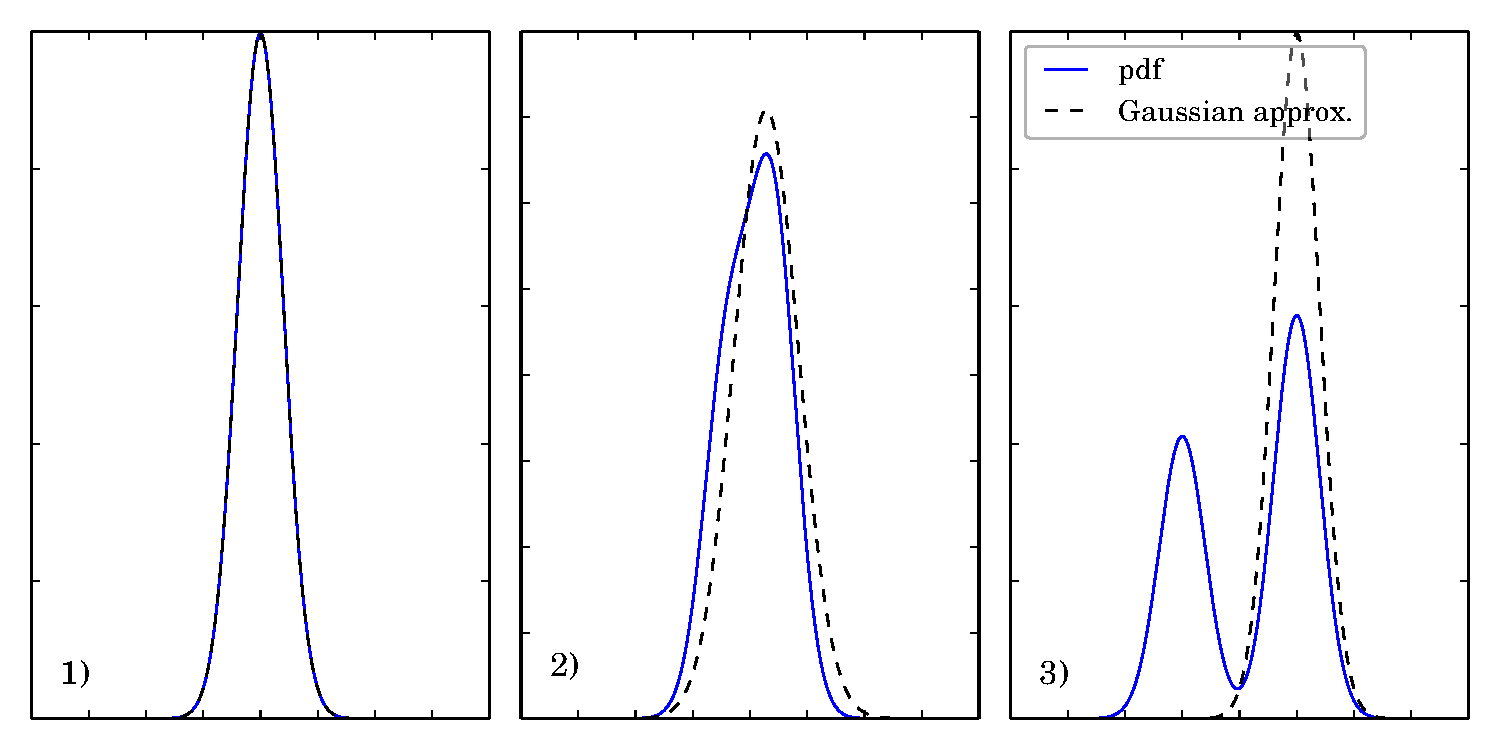
\includegraphics[keepaspectratio,width=\textwidth,height=200pt]{figures/gaussian_approximation.pdf}
\label{gaussian_approximation}
\end{figure}

\end{frame}

\begin{frame}

\frametitle{Bibliography}
\label{bibliography}

% Bibliography slide 


\bibliographystyle{unsrt}
\bibliography{stats_part03}


\end{frame}

\mode<all>
\input{mmd-beamer-footer}

\end{document}\mode*

